\section{Adding and Editing Events}


\subsection{Adding a New Event}

To add a new event to the system, select ``New Event'' from the drop-down menu in the Toolbar. You will be directed to the ``Add New Booking'' form. Fill out all the required fields in the form, and click ``Continue''. If you want to clear the form, click 'Reset'.

If you are not an Administrator, you may only add \textit{tentative} (\textit{requested}) events; an Administrator will need to confirm your room booking.

If you are an Administrator or a Staff member, you may add events on behalf of any Partner. If you are a Partner, you may add events only on your own organization's behalf.

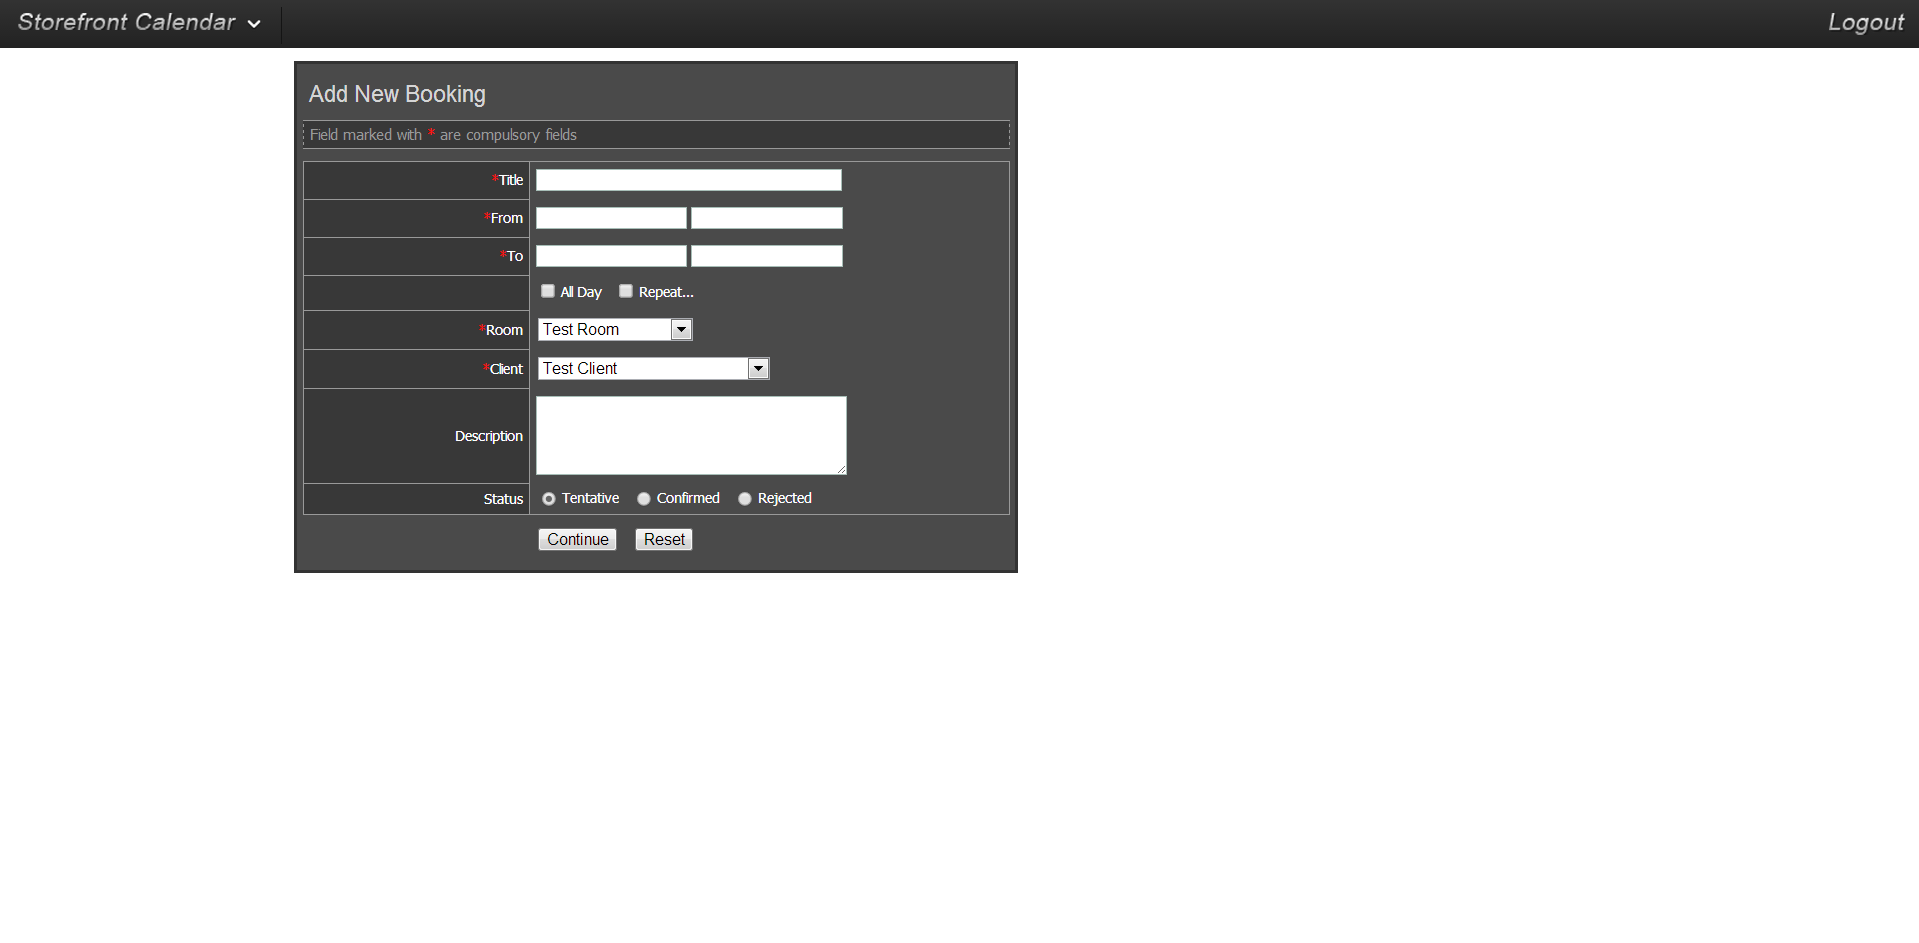
\includegraphics[width=\linewidth]{screenshots/img_addevent}

\newpage


\subsection{Editing an Existing Event}

To edit an existing event, select ``Edit Event'' from the drop-down menu in the Toolbar. You will be directed to the ``Edit Bookings'' form. Fill out all the required fields in the form, and click ``Save''. If you want to delete the event, click ``Delete''.

If you are not an Administrator and you edit a non-tentative booking, it will become tentative; an Administrator will need to confirm the new booking details.

If you are an Administrator or a Staff member, you may edit events on behalf of any Partner. If you are a Partner, you may edit only your own organization's events.

Shortcut: You can also edit an event by double left-clicking on it. If you are a Partner and do not own the event, the ``Edit Bookings'' form will still be brought up, however you will only be able to edit bookings you own.

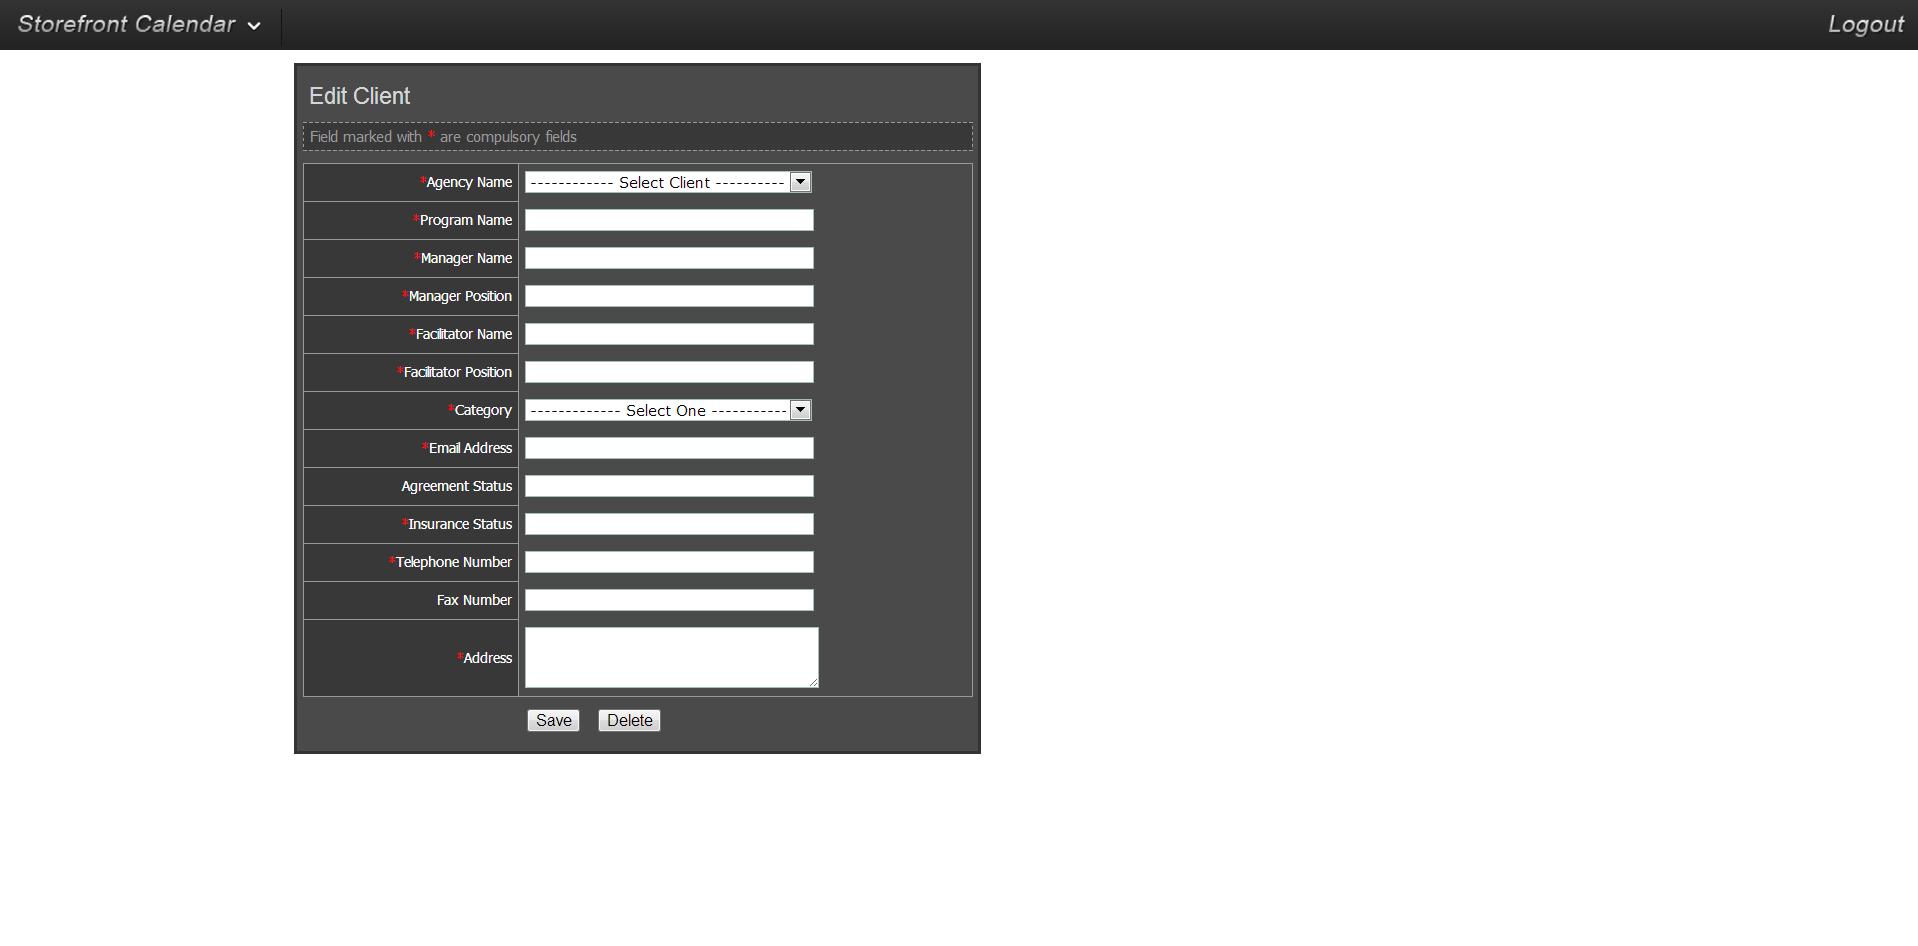
\includegraphics[width=\linewidth]{screenshots/img_editevent}

